\documentclass[11pt]{article}
\usepackage[final]{acl}
\usepackage{times}
\usepackage{latexsym}
\usepackage[T1]{fontenc}
\usepackage[utf8]{inputenc}
\usepackage{microtype}
\usepackage{inconsolata}
\usepackage{graphicx}
\usepackage{booktabs}
\usepackage{multirow}
\usepackage{amsmath}
\usepackage{amssymb}
\usepackage{xspace}

\newcommand{\qwen}{Qwen2.5-VL-7B\xspace}
\newcommand{\llava}{LLaVA-NeXT-7B\xspace}
\newcommand{\cls}[1]{\textsc{#1}}

\title{Type-Aware Failure Prediction for Chart and Diagram\\Reasoning in Vision-Language Models: Mid-Term Report}

\author{Yash More, Naman Singhal, Shrish Kadam, Sanjith Ganapathi \\
  \texttt{\{yash.more, naman.s, shrish.kadam\}@research.iiit.ac.in}, \texttt{sanjith.ganapathi@students.iiit.ac.in} \\
  International Institute of Information Technology, Hyderabad}

\begin{document}
\maketitle

\begin{abstract}
When a vision-language model (VLM) answers a chart question wrongly, it may have
misread the figure (a \emph{structural} failure) or stated something the figure
does not contain (a \emph{fabrication}). We ask whether the two are
distinguishable in the model's internal state before it generates an answer. We
ran \qwen and \llava over the 2,500 ChartQA test questions and cached pooled
activations at every decoder layer from the same forward pass that produced each
answer. A linear probe on the last prompt token predicts whether the answer
will be wrong with test AUROC 0.932 for Qwen (0.786 for a surface-feature
baseline) and 0.798 for LLaVA (0.608). Labelling Qwen's 317 errors showed that
fabrication is essentially absent from ChartQA (1 of 317), and that 35\% of the
scored errors are not errors at all. We therefore built a synthetic bar-chart
arm that asks about categories absent from the chart. Both models almost never
refuse such questions (15 refusals in 1,200 for Qwen, 0 for LLaVA), yet both
represent that the asked category is missing (probe AUROC 0.96 to 1.00, with
text-only and image-only controls at chance). In Qwen, probes for misreads and
for missing-bar fabrications are largely type-specific (own-type AUROC 0.887 and
1.000; cross-type 0.594 and 0.576). In LLaVA the missing-bar signal is specific
but the misread probe is not: it fires more on fabrications (0.879) than on
misreads (0.776), and a one-number chart feature predicts LLaVA's misreads
better than its activations. The Type Separability Hypothesis is thus supported
for one model and only partly for the other.
\end{abstract}

\section{Introduction}

VLMs are increasingly used to read charts, plots and diagrams whose answers feed
decisions. When such a model answers incorrectly, it can be wrong in two
mechanically different ways. It may have \textbf{misread the figure}: picked the
wrong bar, misjudged an axis tick, traced the wrong edge. The correct answer was
in the image, and a more careful look might recover it. Or it may have
\textbf{fabricated}: stated a value or label that appears nowhere in the figure.
Looking again will not help, and the answer should be withheld.

Reliability tooling today collapses both into one ``do not trust'' verdict.
Abstaining on everything discards recoverable answers; re-querying everything
spends compute on answers that were never grounded. Our project asks whether
the distinction is visible in the model's internal state \emph{before}
generation, and whether knowing it is worth anything.

\paragraph{Refined problem statement.} Let $x=(I,q)$ be a chart image and a
question, and $\hat{y}$ the answer a frozen VLM generates greedily. Let
$h_{\ell}^{p}(x)\in\mathbb{R}^{d}$ be the model's hidden state after decoder
layer $\ell$, pooled at prompt position $p$, computed in the prefill pass that
precedes the first answer token. Each wrong answer carries a failure type
$t\in\{\cls{structural},\cls{fabrication}\}$ determined from $\hat{y}$ and the
figure. We test (i) whether $\Pr(\hat{y}\text{ wrong}\mid h)$ and
$\Pr(t\mid h, \hat{y}\text{ wrong})$ can be estimated by linear probes on
$h_\ell^p$ better than by surface features of the input, and (ii) whether the
probe for one failure type also responds to the other (cross-transfer). Later
stages (E4, E5) test whether the type determines which repair works.

\paragraph{Progress summary.} All planned inference and activation caching is
complete for both models on ChartQA and on two synthetic pilots
(Section~\ref{sec:setup}). The binary and type probes (E1, E3) are trained with
surface baselines (a partial E2). Section~\ref{sec:chartqa} reports the
naturalistic arm, including why it cannot supply fabrication examples;
Section~\ref{sec:synth} the synthetic arm built in response;
Section~\ref{sec:discussion} what the results say about the hypothesis; and
Section~\ref{sec:plan} the plan for the remaining weeks.

\section{Background and Related Work}

\subsection{Pre-generation failure detection}
\citet{kogilathota2026halp} establish that hallucination risk in VLMs is
readable from internal representations in a single forward pass, without
decoding, reaching up to 0.93 AUROC across eight models. Two of their findings
shaped our design: the most informative representation family varies by
architecture, with \qwen best served by visual-only features at roughly 0.79
AUROC, where most models rely on late query-token states.
\citet{zhang2026vibprobe} localise the signal further, isolating
hallucination-relevant attention heads through a variational information
bottleneck and using probe gradients to intervene at inference time. Both works
address binary object hallucination on natural photographs. Neither asks
whether distinct kinds of failure are internally distinguishable.

\subsection{Evidence that failure types differ mechanistically}
\citet{liu2026dualpathway} apply activation patching across five VLMs and
identify a visual grounding pathway supporting correct predictions alongside a
separate hallucination pathway driving erroneous ones, the former at
mid-to-late depths and the latter concentrated at early layers and network
boundaries. The identified circuit transfers selectively to relational but not
attribute hallucination. That selectivity is the closest existing evidence that
hallucination is not one internal phenomenon, and is the empirical basis for
our hypothesis. It also motivates probing across the full depth of the network,
since the two pathways do not occupy the same layers.

\subsection{Chart and diagram reasoning}
ChartQA \citep{masry2022chartqa} remains the standard benchmark for chart
question answering with visual and logical reasoning. \citet{rani2025radar}
contribute chart, question, reasoning-step and attribution annotations,
identifying which regions justify a model's answer.
\citet{iyengar2026dragon} assemble diagram QA instances across six source
datasets, annotating the minimal regions required to verify each answer, and
find that correct answers do not guarantee a model grounded its reasoning in the
supporting regions. Both resources annotate \emph{where a model should look}.
Neither labels \emph{how a model failed}, which is the supervision signal we
need.

\subsection{Error taxonomies and visual self-correction}
\citet{ashurytahan2026errormap} argue that benchmark accuracy reports whether a
model fails but not why, and build an LLM-judge pipeline for taxonomy
construction across 35 datasets and 83 models. Their setting is text-only LLMs;
we borrow the methodology, not the taxonomy. \citet{li2026visualselfrefine}
propose Visual Self-Refine, in which a chart-parsing model emits pixel-level
localisations, visualises them, and feeds them back to itself to correct its own
perception errors. Making a model re-examine a figure is therefore established;
what is untested is whether the \emph{appropriate} repair depends on which
failure occurred.

\subsection{Probe validity}
Two results define our standard of evidence. \citet{sahoo2026linearprobes}
report probes separating reasoning types at 100\% accuracy with well-separated
geometry, then show the separation was driven entirely by format confounds,
collapsing to chance once source identity, option count and response length were
residualised out. \citet{yuan2026hiddenerror} report the healthy contrast, a
hidden-state probe at 0.95 AUROC against a text-surface classifier at 0.59, but
find that four interventions built on that signal failed: the signal was
diagnostic, not causal. Two lessons follow: a probe result is uninterpretable
without a surface baseline, and detection does not imply a usable intervention.

\subsection{Positioning}
Pre-generation detection is binary and targets natural images; mechanistic
type-selectivity has been shown for object hallucination, not structured-image
reasoning; chart resources annotate evidence regions, not failure types; and
visual self-correction is applied uniformly. Our work sits in the intersection:
failure-\emph{type} prediction on structured images, and whether that type
should determine the repair.

\section{Hypothesis}

\textbf{Type Separability Hypothesis.} The pre-generation internal state
preceding a structural misreading is linearly distinguishable from the state
preceding a fabrication, because the former is a precision-limited perceptual
failure while the latter reflects generation ungrounded in the image. We test
this rather than assume it: a misread bar height may be a higher-precision
instance of the same perceptual failure, and the design treats a collapse of the
two classes as a reportable outcome.

\section{Experimental Setup}
\label{sec:setup}

\subsection{Models and inference}
We use two frozen open VLMs: \qwen \citep{bai2025qwen25vl} and LLaVA-NeXT with
a Mistral-7B language model (\texttt{llava-v1.6-mistral-7b};
\citealp{liu2024llavanext}). ChartGemma, the stretch goal, is dropped. Every
question is asked with the standard ChartQA suffix ``Answer the question using a
single word or phrase.'', decoded greedily (at most 32 new tokens), in fp16 with
SDPA attention on two RTX 2080 Ti GPUs. Hardware, library versions and settings
are frozen and recorded with every run, because a different GPU kernel can
change the generated answer and decouple the cached activations from the answer
that was labelled. Answers are scored by ChartQA relaxed accuracy (numeric
answers within 5\% of the gold; strings by exact match).

\subsection{Activation caching}
Activations are captured by forward hooks \emph{during the same} \texttt{generate()}
call that produced the answer, from its prefill pass, so every vector belongs to
the labelled answer. Layer $\ell$ is the residual stream after decoder block
$\ell$. We cache every layer (Qwen: 28 layers, $d=3584$; LLaVA: 32 layers,
$d=4096$) at four pooled positions: \textbf{vision\_mean} and
\textbf{vision\_max} (mean and elementwise max over the image tokens),
\textbf{query\_last} (the final prompt position, i.e.\ the state from which the
first answer token is predicted) and \textbf{query\_mean} (mean over the text
tokens of the prompt). Pooling is what makes full-depth caching affordable: the
image contributes on average 584 tokens per question for Qwen and 2,212 for
LLaVA. Caches are stored in fp16 (1.5 GB for Qwen and 2.0 GB for LLaVA on the
ChartQA test set).

\subsection{Probes}
\label{sec:probes}
A probe is an $L_2$-regularised logistic regression on one pooled vector. For a
chosen layer $\ell$ and position $p$, the input $h=h_\ell^p(x)$ is z-scored with
the mean and standard deviation of the \emph{training} items only, and the probe
outputs a score $s(x)=w^{\top}h+b$, trained by minimising the logistic loss plus
$\tfrac{\lambda}{2}\lVert w\rVert^2$ (L-BFGS; the intercept is not penalised).
There are $d+1$ parameters (3,585 for Qwen, 4,097 for LLaVA), which is more than
the number of positive training examples in every task, so $\lambda$ is
selected from $\{1,10,10^2,10^3,10^4\}$. Probes are scored by AUROC: the
probability that a randomly chosen positive item receives a higher score than a
randomly chosen negative one. We train two kinds:

\textbf{Single-split sweep probes} (binary, ChartQA structural, and
absent-versus-present on synthetic data). Items are split 60/20/20 by
\emph{figure} (hashed, seed 42), so no chart appears in two splits. Every
(position, layer, $\lambda$) cell is fitted on train and scored on validation;
the best cell is chosen on validation only, and the test set is scored once.

\textbf{Cross-validated type probes} (the E3 matrix on synthetic data, where
misreads are too few for a single held-out split). Items are assigned to five
folds by figure. Within each outer fold, layer and $\lambda$ are chosen by an
inner cross-validation over the other four folds, and the probe then scores the
held-out fold. Every item thus receives an out-of-fold score from a probe that
never saw its chart. Position is fixed to query\_last in advance.

All intervals are 95\% percentile intervals from a bootstrap that resamples
whole figures (2,000 draws), because questions on the same chart are correlated.
Every probe is reported next to a baseline that sees no activations.

\section{Naturalistic Arm: ChartQA}
\label{sec:chartqa}

\subsection{Accuracy}
Table~\ref{tab:acc} gives relaxed accuracy on the ChartQA test set (1,250
human-written and 1,250 machine-augmented questions over 1,509 charts). Qwen is
wrong on 317 questions and LLaVA on 1,178.

\begin{table}[t]
\centering\small
\begin{tabular}{lccc}
\toprule
Model & Overall & Human & Augmented \\
\midrule
\qwen & 87.3 & 79.8 & 94.8 \\
\llava & 52.9 & 44.6 & 61.1 \\
\bottomrule
\end{tabular}
\caption{Relaxed accuracy (\%) on ChartQA test.}
\label{tab:acc}
\end{table}

\subsection{Labelling Qwen's errors}
The proposal planned two classes plus \cls{ambiguous}. A pilot of 20 errors
showed that this forced many items into \cls{ambiguous} for reasons unrelated to
the model, so the team adopted five labels: \cls{structural} (the answer is
explained by misreading the figure: wrong bar or series, misread digits,
imprecise reading, miscounting), \cls{fabrication} (content the figure does not
support), \cls{computation} (inputs read correctly, arithmetic or logic wrong),
\cls{not\_an\_error} (the answer is actually right: an equivalent format, a
wrong gold answer, or a valid reading of an ambiguous question) and
\cls{ambiguous}. Only \cls{structural} and \cls{fabrication} train type probes.
All 317 errors were labelled by an LLM annotator (Claude) that saw only the
chart image, question, gold answer and model answer, following the written
rubric; the planned two-person human agreement check ($\kappa>0.6$ on 200 items)
has not yet been run.

\begin{table}[t]
\centering\small
\begin{tabular}{lrp{3.3cm}}
\toprule
Label & $n$ & Breakdown \\
\midrule
\cls{not\_an\_error} & 112 & 51 format, 38 valid reading, 23 wrong gold \\
\cls{computation} & 93 & \\
\cls{structural} & 71 & \\
\cls{ambiguous} & 40 & 14 question, 11 wrong gold, 12 other, 3 unreadable \\
\cls{fabrication} & 1 & \\
\bottomrule
\end{tabular}
\caption{Labels for Qwen's 317 ChartQA test errors.}
\label{tab:labels}
\end{table}

Table~\ref{tab:labels} gives two findings. First, \textbf{fabrication is
essentially absent} from Qwen's ChartQA errors: one item in 317. ChartQA
questions are written about content the chart contains, so a capable model
rarely has occasion to invent content; its errors are misreads and arithmetic.
The naturalistic arm therefore cannot supply fabrication examples, which is the
risk the synthetic arm was planned for. Second, \textbf{35\% of the scored
errors are not errors}: most often the answer is correct in another format
(``1:2'' for 0.5), the gold answer is wrong, or the question admits the model's
reading. This matters for every probe trained on relaxed-accuracy labels.

\paragraph{What the error types look like.} Examples from the labels, with the
annotator's rationale paraphrased:
\begin{itemize}\itemsep0pt
\item \cls{structural} (71, 22\%): a pie chart with seven labelled sectors
counted as six; the adjacent 2017 bar reported instead of the asked 2018 bar;
the top of a stacked segment reported instead of its height; a reversed
comparison of two bars of similar length.
\item \cls{computation} (93, 29\%, the largest class of real errors): every
input is printed and readable, but the operation is wrong, e.g.\ a ratio of
levels (83/11) where the question asks for a ratio of changes, a sum over four
printed values that matches no subset of years, or picking the larger of two
printed changes wrongly.
\item \cls{not\_an\_error} (112, 35\%): \emph{format}: 0.95 for a gold of 95\%,
``increase'' for ``increasing'', or the same bar named by a different colour
word; \emph{gold wrong}: the model's 28/19 = 1.474 is the correct ratio of the
two bars while the gold 1.18 matches no ratio on the chart; \emph{valid
reading}: a question that names no year, answered for the latest year while the
gold uses the first.
\item \cls{ambiguous} (40, 13\%): both the gold and the model are wrong (11), the
question has several readings and the model fits none (14), the needed value is
unreadable, e.g.\ two near-identical shades of teal (3), or a misread cannot be
told apart from an arithmetic slip (12, ``other'').
\item \cls{fabrication} (1): pie slices of 35, 40, 13 and 11, where the
answer 75 is a sum of two slices; the model's 55 matches no slice and no sum.
\end{itemize}
Only 22\% of Qwen's scored errors are figure misreads; nearly as many are
arithmetic or reasoning slips, which the two-class taxonomy of the proposal did
not provide for.

\subsection{Predicting whether the answer is wrong (E1)}
\label{sec:e1}

\begin{table}[t]
\centering\small
\begin{tabular}{lcc}
\toprule
 & Probe & Surface \\
\midrule
Qwen, all errors & 0.877 {\scriptsize[.83,.92]} & 0.715 \\
Qwen, without \cls{not\_an\_error} & \textbf{0.932} {\scriptsize[.90,.96]} & 0.786 \\
LLaVA, all errors & 0.798 {\scriptsize[.76,.84]} & 0.608 \\
\midrule
Qwen, structural vs.\ correct & 0.905 {\scriptsize[.84,.97]} & -- \\
\bottomrule
\end{tabular}
\caption{Test AUROC [95\% CI] of the binary probe (wrong vs.\ right) and of the
Qwen structural probe on ChartQA, against a surface-only baseline (question
source, question length, number of image tokens, numeric gold). All selected
query\_last; Qwen layer 21 of 28, LLaVA layer 24 of 32.}
\label{tab:e1}
\end{table}

Table~\ref{tab:e1} reports the binary probe. A sanity probe first confirmed that
each cache decodes what it plainly contains (human-written vs.\ augmented
question: validation AUROC 1.000 for Qwen, 0.999 for LLaVA). For both models the
probe clearly exceeds the surface baseline, with non-overlapping intervals.
Removing Qwen's 112 \cls{not\_an\_error} items raises the probe from 0.877 to
0.932: part of what looked like probe error was label noise. The probe is not
reading question style, which alone predicts errors at 0.68 for Qwen because
80\% of its errors are on human-written questions: within human-written
questions only it reaches 0.895 (Qwen, cleaned) and 0.850 (LLaVA). LLaVA's lower
raw AUROC should not be read as a weaker signal; it is wrong on 47\% of
questions against Qwen's 13\%, so the two probes separate different error sets
at different base rates, and its gap over its own baseline (+0.19) is similar to
Qwen's (+0.15).

\textbf{Which layers.} Figure~\ref{fig:binary} shows validation AUROC by relative
depth. In both models the signal is in the query-side state and builds with
depth: query\_last rises from about 0.70 at the first layer to a plateau over
the last third of the network (Qwen 0.85 to 0.87 over layers 18 to 27, best at
21; LLaVA 0.83 to 0.84 over layers 20 to 28, best at 24). The image-token
positions stay flat at 0.62 to 0.68 at every depth, close to the surface
baseline. This differs from HALP's finding that Qwen is best served by
visual-only features for object hallucination on photographs; for chart errors
the informative state is the one that has already read the question.

\begin{figure}[t]
\centering
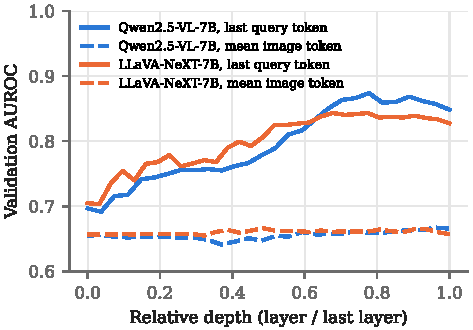
\includegraphics[width=\columnwidth]{figures/binary_by_layer.pdf}
\caption{Binary probe, validation AUROC by relative depth (best $\lambda$ per
layer). Solid: last prompt token; dashed: mean over image tokens.}
\label{fig:binary}
\end{figure}

\textbf{A structural probe on real charts.} Using the 71 \cls{structural} labels
against all correct answers (other labels excluded), a Qwen probe reaches test
AUROC 0.905, again at query\_last, layer 21. With only 13 structural errors in
the test split the interval [0.84, 0.97] is the result, and this probe does not
yet have its own surface baseline. With one fabrication, the corresponding
fabrication probe cannot be trained on ChartQA.

\section{Synthetic Arm}
\label{sec:synth}

\subsection{Design}
The synthetic arm makes fabrication happen on purpose, by asking about
categories that are absent from the chart. Two design constraints come from
earlier checks. (1) A probe comparing ChartQA misreads with synthetic
fabrications would learn ``real vs.\ synthetic chart''. (2) On synthetic data the
question template alone predicts the intended failure type at AUROC 1.000, so a
probe comparing one template with another can read the template. Every contrast
is therefore made \emph{within one question template}, and every outcome is
scored from the model's actual answer, never from what the question was
designed to induce.

\textbf{Pilot 1} rendered 300 bar charts (matplotlib; 4 to 7 bars; six themes
such as fruits or cities; values on 0--50 or 0--100 axes). Each chart is asked
the same question twice, in identical words: once about a bar that is shown
(``What is the value of Mango?'') and once about a plausible name from the same
theme that is not (``\dots of Guava?''). \textbf{Pilot 2} (300 charts, 1,800
questions) added three changes after pilot 1. (i) Category names come in
lookalike pairs (Dubai/Dublin, Eagle/Falcon, Lute/Flute); a chart shows at most
one of a pair, and half the absent questions ask for the partner of a shown bar.
(ii) Three question families, each asked about a shown and a missing name:
\emph{value}, \emph{compare} (``Which is larger, Guava or Apple?'') and
\emph{neighbor} (``Which bar is immediately to the right of Guava?''). Naming any
bar in reply to the last is a fabrication with no numeric escape. (iii) Harder
charts: values never multiples of 5, axes up to 200, sparse ticks. Generation is
deterministic, and both models were run on byte-identical charts.

Answers to missing names are scored as \emph{rejected} (``None''),
\emph{fabricated} (any other number; naming the missing bar, its lookalike or
any bar for neighbor questions), \emph{zero} (``0'') or
\emph{picked-present} (naming the shown bar in a compare question). The team
decided that ``0'' to a value question is a refusal expressed as a number, not a
fabrication: no bar in these charts has zero height, so the model is not
reporting something it read, and Qwen says ``0'' mostly when no bar resembles
the asked name (141 of 157 unrelated names). It still counts as a wrong answer.

\subsection{How the models answered}

\begin{table}[t]
\centering\small
\begin{tabular}{llcc}
\toprule
 & & Qwen & LLaVA \\
\midrule
\multirow{3}{*}{Shown bar, right} & value (P1+P2) & 554/600 & 185/600 \\
 & compare & 300/300 & 209/300 \\
 & neighbor & 294/300 & 255/300 \\
\midrule
\multirow{4}{*}{Missing, value} & rejected & 15 & 0 \\
 & ``0'' & 494 & 232 \\
 & fabricated & 91 & 368 \\
\midrule
Missing, compare & fabricated & 37 & 101 \\
Missing, neighbor & fabricated & 300 & 290 \\
\bottomrule
\end{tabular}
\caption{Synthetic outcomes (pilots 1 and 2). Value rows pool both pilots (600
missing-name questions); compare and neighbor come from pilot 2 (300 each).}
\label{tab:synth}
\end{table}

Table~\ref{tab:synth} summarises the answers. \textbf{Neither model refuses}:
Qwen rejects 15 of 1,200 missing-name questions and LLaVA none. Qwen answers
most missing values with ``0''; when it does invent a number, 57 of its 76
pilot-2 inventions are the value of the lookalike bar, i.e.\ it binds the
missing name to the nearest-looking bar that is present (asked for Dubai, it
reports Dublin). LLaVA invents far more often (368 vs.\ 91), mostly round
numbers near some bar. The models also differ on shown bars: Qwen reads 92\% of
values within tolerance, LLaVA 31\%, because LLaVA snaps its readings to the
nearest gridline (52 becomes 50). This yields four classes for the value
template: \cls{c} correct read, \cls{s} misread (structural), \cls{f} invented
number (fabrication) and \cls{z} ``0'' (Qwen 554/46/91/494; LLaVA
185/415/368/232).

\subsection{Do the models know the bar is missing?}

\begin{table}[t]
\centering\small
\begin{tabular}{lcc}
\toprule
Family & Qwen & LLaVA \\
\midrule
value & 0.999 {\scriptsize(L4)} & 0.977 {\scriptsize(L12)} \\
compare & 0.991 {\scriptsize(L4)} & 0.959 {\scriptsize(L19)} \\
neighbor & 1.000 {\scriptsize(L5)} & 0.996 {\scriptsize(L18)} \\
\midrule
lookalike names only & 0.980--1.000 & 0.922--0.991 \\
text-only baseline & 0.49--0.52 & 0.49--0.52 \\
image-token probe & 0.500 & 0.500 \\
\bottomrule
\end{tabular}
\caption{Test AUROC of probes separating a missing from a shown name under
identical wording (pilot 2; 62 charts per class in test). The image-token probe
is a built-in control: image tokens precede the question, so they cannot see
it.}
\label{tab:absent}
\end{table}

Table~\ref{tab:absent} shows that \textbf{both models represent that the asked
name is missing, although they answer anyway}. Two controls make the result
interpretable. A classifier on the question text alone is at chance, because
every name is a shown bar on some charts and missing on others. Probes on the
image-token positions score exactly 0.500: the image precedes the question in
the prompt and attention is causal, so both questions of a chart receive
identical image vectors. The signal holds for lookalike names, and it appears
early in Qwen (validation 0.99 from layer 2) and later in LLaVA (about layer 9).
The absence probe does not respond to misreads of shown bars (Qwen 0.46, LLaVA
0.51 on shown-bar value questions).

\subsection{Type probes and cross-transfer (E3)}

\begin{table*}[t]
\centering\small
\begin{tabular}{l|cccc|cccc}
\toprule
 & \multicolumn{4}{c|}{\qwen} & \multicolumn{4}{c}{\llava} \\
Probe (trained on) & \cls{s} vs \cls{c} & \cls{f} vs \cls{c} & \cls{z} vs \cls{c} & \cls{f} vs \cls{z} & \cls{s} vs \cls{c} & \cls{f} vs \cls{c} & \cls{z} vs \cls{c} & \cls{f} vs \cls{z} \\
\midrule
structural (\cls{s} vs \cls{c}) & \textbf{0.887} & 0.594 & 0.673 & 0.400 & \textbf{0.776} & 0.879 & 0.987 & 0.215 \\
\quad metadata baseline & 0.814 & 0.557 & 0.515 & 0.543 & 0.512 & 0.522 & 0.486 & 0.537 \\
fabrication (\cls{f} vs \cls{c}) & 0.576 & \textbf{1.000} & 1.000 & 0.286 & 0.680 & \textbf{0.988} & 1.000 & 0.243 \\
\quad metadata baseline & 0.588 & 0.840 & 0.564 & 0.787 & 0.642 & 0.769 & 0.643 & 0.651 \\
invented vs.\ zero (\cls{f} vs \cls{z}) & 0.336 & 0.138 & 0.000 & \textbf{0.984} & 0.520 & 0.226 & 0.000 & \textbf{0.986} \\
\bottomrule
\end{tabular}
\caption{Cross-transfer matrix on synthetic value questions (5-fold CV by chart,
out-of-fold AUROC). Rows: the probe and what it was trained on; columns: the
contrast it is scored on. Bold: each probe on its own task. Metadata baseline:
the same procedure on chart settings only (pilot, axis range, tick density, bar
count, lookalike present, phrasing). 95\% CIs for the bold cells: Qwen
[0.82, 0.94], [1.00, 1.00], [0.97, 0.99]; LLaVA [0.73, 0.82], [0.98, 0.99],
[0.98, 0.99]; for the structural probe on \cls{f} vs \cls{c}, Qwen
[0.55, 0.65], LLaVA [0.85, 0.90].}
\label{tab:matrix}
\end{table*}

Table~\ref{tab:matrix} is the central result. Each probe is trained on one pair
of classes and then scored on every pair. If misreads and fabrications leave
different internal signatures, each probe should be strong on its own task
(bold) and weak on the other failure type.

\textbf{Qwen: largely type-specific.} The structural probe separates misreads
from correct reads (0.887) but barely responds to fabrications (0.594); the
fabrication probe is perfect on its own task and near chance on misreads
(0.576, interval touching 0.5). The structural probe exceeds its metadata
baseline by a modest 0.07 with overlapping intervals: much of Qwen's misread
risk is chart difficulty visible in the settings (0--200 axes with sparse ticks
account for most misreads).

\textbf{LLaVA: the misread signal is not type-specific.} Its structural probe
fires \emph{more} on fabrications (0.879) and on ``0'' answers (0.987) than on
its own task (0.776). It behaves like a general ``this answer is not grounded''
direction, strongest when there is no bar at all. Moreover, because LLaVA snaps
to gridlines, the distance of the true value from the nearest multiple of 10
alone predicts its misreads at 0.852, above the probe; for Qwen the same number
gives only 0.616, far below its probe. (This feature was chosen after seeing
LLaVA's rounding, so it is a diagnostic rather than a pre-registered baseline.)

\textbf{In both models the ``fabrication'' probe is a missing-bar detector.} It
scores ``0'' answers exactly as high as invented numbers (\cls{z} vs \cls{c}
1.000) and even ranks them above (\cls{f} vs \cls{z} below 0.3). What separates
an invented number from ``0'' is decodable (0.984, 0.986), but only in the last
layers (Qwen 22 to 27, LLaVA 23 to 30), where it largely reads out the answer
about to be produced rather than giving an early warning.

\textbf{Which layers.} Figure~\ref{fig:types} shows own-task AUROC by relative
depth. The missing-bar signal saturates early (Qwen by layer 3, LLaVA by about
layer 8). The misread signal builds gradually and peaks in the last third
(layers chosen by inner CV: Qwen 16 to 25, LLaVA 20 to 30).

\begin{figure}[t]
\centering
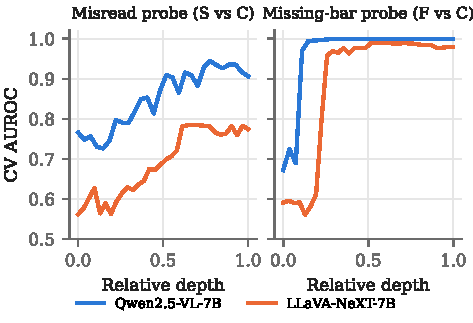
\includegraphics[width=\columnwidth]{figures/type_probes_by_layer.pdf}
\caption{Type probes on synthetic value questions: out-of-fold AUROC on their
own task by relative depth ($\lambda$ chosen per fold by inner CV).}
\label{fig:types}
\end{figure}

\section{Discussion}
\label{sec:discussion}

\paragraph{Is the hypothesis supported?} Partly. For \qwen, the state before a
misread and the state before a missing-bar fabrication are linearly
distinguishable, and each probe is largely blind to the other failure type. For
\llava only one direction holds: the missing-bar signal is specific, but the
misread probe captures a general lack of grounding that is strongest on
fabrications, and a chart-level feature explains its misreads better. Under the
criterion we set in the proposal (``strong cross-transfer indicates one signal
wearing two labels''), LLaVA shows exactly that, from the structural side.

\paragraph{What the fabrication signal is.} With our data, a fabrication is
defined by the missing category, so ``predicting fabrication'' and ``detecting
that the asked category is missing'' cannot be separated. The finding we can
state is that both models encode, early and linearly, that the question is about
something not on the chart, and then answer it anyway. This is the signal a
controller needs: it identifies exactly the questions where re-reading cannot
help and abstention is the right repair.

\paragraph{How the models differ.} Qwen is accurate (87\% on ChartQA, 92\% on
synthetic reads), rarely invents numbers, and when it does it binds the missing
name to a lookalike bar. LLaVA is less accurate (53\% and 31\%), reads coarsely
to gridlines, and invents numbers four times as often. Qwen forms the
missing-bar representation within its first few layers; LLaVA forms it in the
first third. Both concentrate error information in the query-side state of the
last third of the network rather than in the image tokens.

\paragraph{Validity.} Every number above sits next to a baseline with no access
to activations: a surface baseline on ChartQA, a text-only baseline and an
image-token control on synthetic data, and a metadata baseline for the type
probes. The image-token control is exact by construction, which rules out
leakage through the image. Remaining threats are listed in
Section~\ref{sec:limits}.

\section{Progress Against Plan and Timeline}
\label{sec:plan}

\paragraph{Done.} Inference and full-depth caching for both models on ChartQA
test (2,500), ChartQA validation (960, Qwen) and both synthetic pilots (2,400);
Qwen error labels (317); E1 for both models with surface baselines; the E3
matrix for both models on synthetic data; the within-source and
image-token controls.

\paragraph{Changed.} The LLM judge was replaced by an LLM annotator with a
five-label rubric (adding \cls{computation} and \cls{not\_an\_error}); synthetic
fabrication is induced with missing categories and lookalike names, while the
proposal's out-of-range quantities are not yet implemented; the planned
fabricated-versus-rejected contrast was replaced by missing-versus-shown, since
neither model rejects often enough to train it; ChartGemma is dropped.

\paragraph{Go/no-go (30 Sep).} The probes separate the types for Qwen and the
missing-bar signal survives every control in both models, so the second half
pursues E4 and E5 rather than a purely negative write-up.

\paragraph{Remaining.}
\begin{itemize}\itemsep0pt
\item \textbf{Oct 1--8:} human agreement check ($\kappa$ on 200 items, two
annotators); labels for LLaVA's 1,178 ChartQA errors; residualised probes (E2)
and a surface baseline for the ChartQA structural probe.
\item \textbf{Oct 1--15:} E4 cross-intervention matrix (question-conditioned
crop, verify prompt, abstain) on synthetic items, whose bar geometry is recorded
at render time, for both models.
\item \textbf{Oct 16--25:} E5 controller from the binary and missing-bar probes;
risk--coverage and AURC against binary selective prediction and the oracle.
\item \textbf{Oct 26--31:} final report.
\end{itemize}

\section{Limitations}
\label{sec:limits}

The ChartQA labels come from a single LLM annotator and have not yet passed the
human agreement check. Fabrication is absent from ChartQA, so the type contrast
rests on synthetic bar charts and on one question template, where fabrication
coincides with a missing category. Qwen has only 46 synthetic misreads, and the
two models' type matrices rest on very different class balances. The ChartQA
structural probe has 13 positives in test and no surface baseline yet. Probes
are linear and diagnostic; whether the signals support a useful intervention is
the question E4 and E5 must answer.

\bibliography{references}

\end{document}
